% ==========================================================================
% Evaluation on real glioma anatomy -- results
% (continues the section opened in 06-real-data-setup.tex)
% ==========================================================================

\subsection{Surrogate Accuracy}
\label{sec:results_main}

Table~\ref{tab:main_results} reports every surrogate on the same
$468$ patient--configuration columns, Table~\ref{tab:per_case} splits the
same numbers by irradiation geometry, and Fig.~\ref{fig:forecasts} shows the
forecasts for one patient.

\begin{table}[H]
\caption{Forecast accuracy on the real cohort. ``Test'' is the relative RMSE on
$(35,80]$, median over $468$ patient--configuration columns and 20 noisy
assimilation realisations; IQR is its inter-quartile range across columns;
$|e_{80}|$ is the absolute final-time error; ``Train'' is the in-window fit
(the observation noise floor is 2\,\%); $\bar\Phi$ is the realised physics
share of Eq.~\eqref{eq:phi}.}
\label{tab:main_results}
\centering\scriptsize
\setlength{\tabcolsep}{4pt}
%
\begin{tabular}{lrrrrr}
\hline
\textbf{Surrogate} & \textbf{Test} & \textbf{IQR} & $\bm{|e_{80}|}$ & \textbf{Train} & $\bm{\bar\Phi}$ \\
 & (\%) & & (\%) & (\%) & \\
\hline
ODE (logistic, $q{=}1$) & 25.62 & 16.8 & 31.0 & 1.63 & 1.00 \\
ODE (volumetric, $q{=}2/3$) & 23.17 & 13.5 & 25.1 & 1.60 & 1.00 \\
ODE (trained $q$) & 26.05 & 15.4 & 31.2 & 1.57 & 1.00 \\
NODE & 28.49 & 19.0 & 34.7 & 1.32 & 0.00 \\
PI-NODE $(\omega,s_r){=}(0.05,0.10)$ & \textbf{20.78} & \textbf{25.0} & \textbf{24.5} & \textbf{1.73} & \textbf{0.18} \\
PI-NODE $(\omega,s_r){=}(0.20,0.05)$ & 21.87 & 13.2 & 26.2 & 1.44 & 0.36 \\
PI-NODE, volumetric backbone & 21.49 & 14.0 & 26.4 & 1.44 & 0.39 \\
CPI-NODE $\lambda{=}0.4$ & 28.00 & 17.9 & 35.2 & 1.34 & 0.61 \\
CPI-NODE $\lambda{=}0.4$, identified & 24.64 & 13.3 & 29.2 & 1.42 & 0.91 \\
CPI-NODE, identified, trained $q$ & 24.40 & 12.6 & 29.2 & 1.41 & 0.91 \\
GPI-NODE (learned gate) & 24.24 & 13.0 & 26.9 & 1.56 & 0.92 \\
GPI-NODE, identified & 23.77 & 12.8 & 26.9 & 1.47 & 1.00 \\
GPI-NODE, identified + autonomous & 23.77 & 12.8 & 27.1 & 1.46 & 1.00 \\
Bounded closure only ($\lambda{=}1$) & 26.05 & 90.7 & 20.5 & 21.29 & 0.00 \\
Bounded closure only, autonomous & 30.21 & 78.6 & 40.8 & 21.30 & 0.00 \\
\hline
\end{tabular}

\end{table}

\begin{table}[H]
\caption{Forecast relative RMSE (\%) by irradiation geometry; median over
patients and realisations. The best entry in each column is bold.}
\label{tab:per_case}
\centering\scriptsize
\setlength{\tabcolsep}{5pt}
%
\begin{tabular}{lrrrr}
\hline
\textbf{Surrogate} & \textbf{Full} & \textbf{Narrow} & \textbf{Slight} & \textbf{Strong} \\
\hline
ODE (logistic, $q{=}1$) & 38.1 & 25.9 & 29.7 & 18.9 \\
ODE (volumetric, $q{=}2/3$) & \textbf{29.8} & 27.0 & 21.8 & 20.0 \\
ODE (trained $q$) & 35.6 & 27.1 & 28.3 & 19.9 \\
NODE & 47.4 & 29.4 & 32.1 & 21.8 \\
PI-NODE $(\omega,s_r){=}(0.05,0.10)$ & 39.0 & 14.2 & 36.9 & 12.3 \\
PI-NODE $(\omega,s_r){=}(0.20,0.05)$ & 32.9 & 20.1 & 22.9 & 18.2 \\
PI-NODE, volumetric backbone & 34.5 & 20.4 & 23.3 & 17.5 \\
CPI-NODE $\lambda{=}0.4$ & 40.4 & 26.6 & 30.6 & 20.9 \\
CPI-NODE $\lambda{=}0.4$, identified & 34.2 & 26.0 & 24.1 & 21.1 \\
CPI-NODE, identified, trained $q$ & 34.1 & 25.1 & 24.1 & 20.4 \\
GPI-NODE (learned gate) & 31.3 & 26.4 & 22.7 & 21.2 \\
GPI-NODE, identified & 30.0 & 27.2 & 20.5 & 21.3 \\
GPI-NODE, identified + autonomous & 30.0 & 27.0 & \textbf{20.4} & 21.3 \\
Bounded closure only ($\lambda{=}1$) & 100.0 & \textbf{9.8} & 70.2 & \textbf{9.1} \\
Bounded closure only, autonomous & 100.0 & 31.8 & 29.2 & 23.8 \\
\hline
\end{tabular}

\end{table}

\begin{figure}[t]\centering
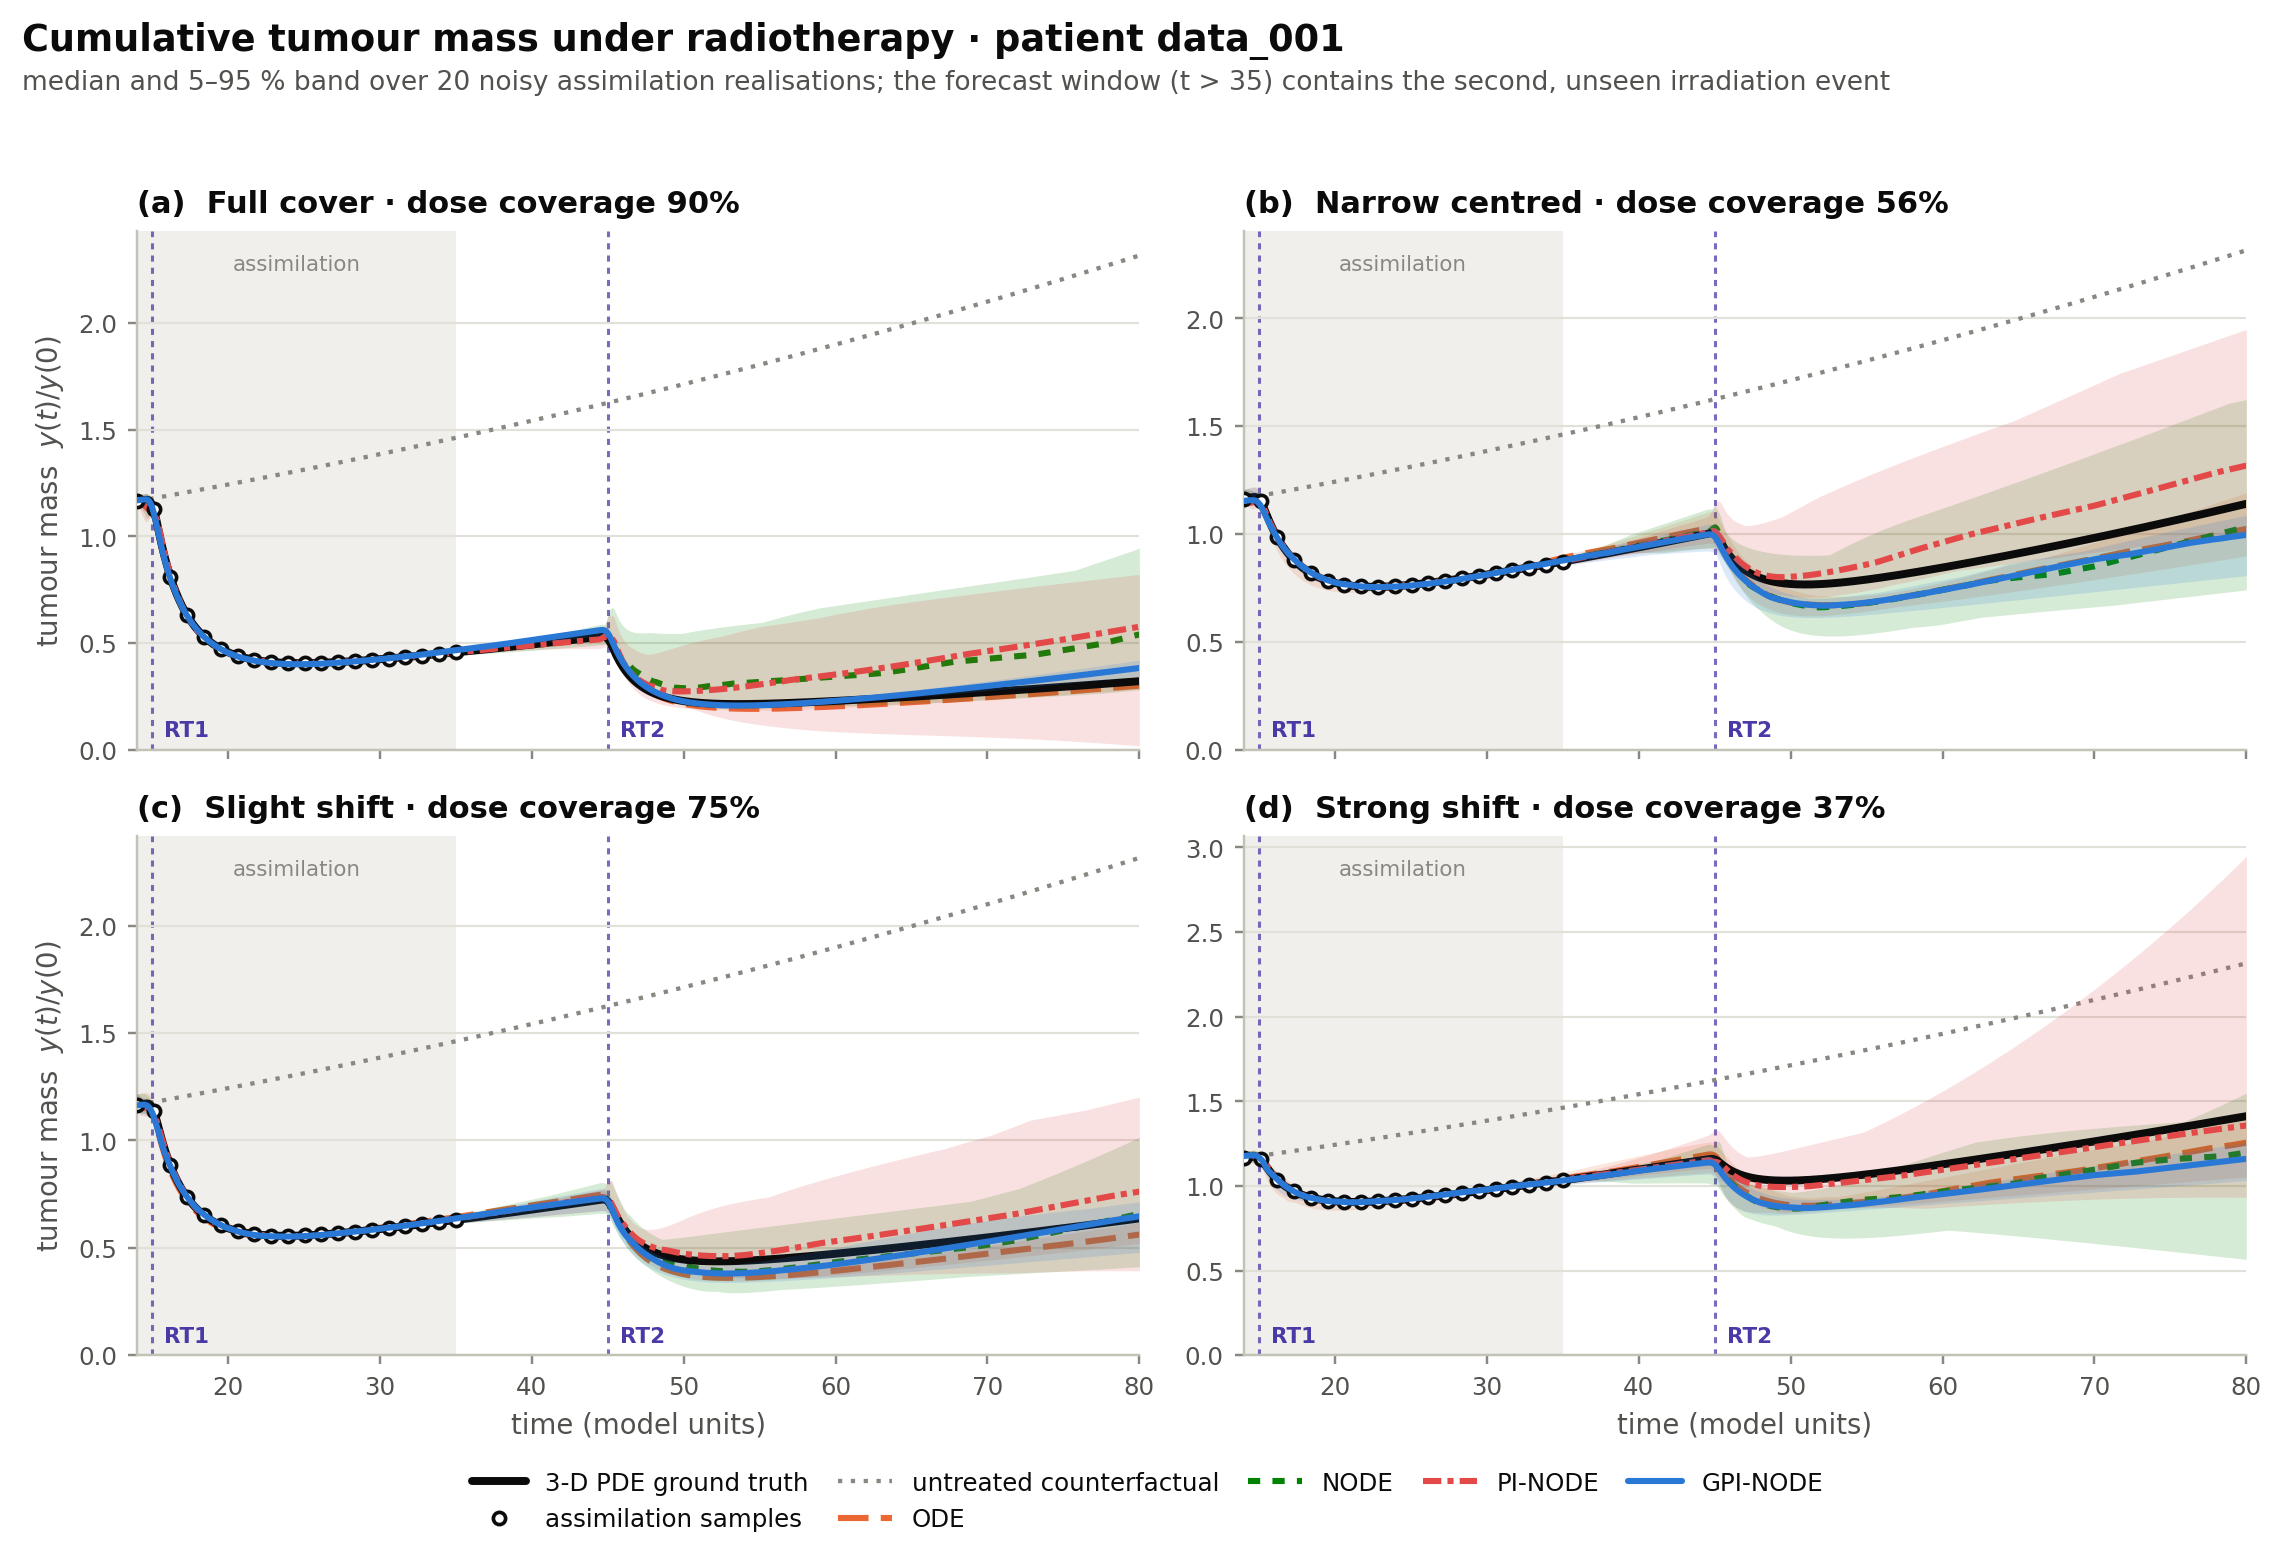
\includegraphics[width=1.0\textwidth]{figures/f5_forecasts.png}
\caption{Cumulative tumour mass for one patient under the four irradiation
geometries. Black is the three-dimensional reference, circles the sparse noisy
observations used for assimilation, and the bands are the 5--95\,\% range over
20 noisy realisations. The forecast window contains the second, unseen
fraction. Every model reproduces the assimilation window; they separate only
after it.}
\label{fig:forecasts}\end{figure}

\paragraph{The paper's central claim is confirmed, and by a wider margin than on
the phantom.} On the two geometry-mismatched configurations --- the situations
this work is about --- a learned closure is decisively better than any purely
mechanistic surrogate: on \texttt{narrow\_centered} the best mechanistic model
reaches 25.9\,\% against 9.8\,\% for a
bounded learned closure, and on \texttt{strong\_shift}
18.9\,\% against 9.1\,\%. That is a factor of
$2$--$3$, on real anatomy, for exactly the effect the closure was introduced to
capture.

\paragraph{The optimum inverts with the geometry.} Where the field covers the
tumour the purely mechanistic model wins and an unconstrained closure fails
outright; where the field is under-sized or displaced the ordering reverses
(Table~\ref{tab:per_case}). The realised physics share of the per-configuration
winner runs from $\Phi\approx1$ to $\Phi\approx0$ within the same cohort. For a
\emph{bounded} closure this makes a single $\lambda$ costly --- forcing one
value everywhere costs up to 148\,\% on the worst
configuration --- which is the argument for the state-dependent gate of
Eq.~\eqref{eq:gate}. For the \emph{unbounded} closure of
Eq.~\eqref{eq:pinode_weighted} a single setting suffices
(8\,\%), precisely because an unbounded closure is
free to adapt itself per patient without help from the weight. Bounding it buys
identifiability and costs that adaptivity.

\paragraph{PI-NODE's overall advantage is not statistically resolved, and it is
the least reliable model.} Its median is the lowest
(20.78\,\%), but a paired Wilcoxon test over the $468$ columns
--- every method sees the same columns and the same noise --- does not separate
it from the volumetric mechanistic model, from its own retuned variant, or from
the gated form proposed here ($p$ between $0.4$ and $0.7$). It also carries by
far the widest spread across the cohort, visible directly as the broad band in
Fig.~\ref{fig:forecasts}. The gated, identified form matches it within noise at
roughly half the inter-quartile range, and reports a calibrated $\lambda$ where
$(\omega,s_{r})$ reports nothing. The honest claim for the replacement is
therefore identifiability and reliability at no significant accuracy cost, not
an accuracy win.

\paragraph{Most of the error is estimation, not model inadequacy.}
Fitting each backbone to the entire noise-free trajectory leaves an irreducible
residual of only 6.96\,\% (logistic) and 6.79\,\%
(volumetric); the assimilated models score several times that
(Fig.~\ref{fig:error_budget}). The dominant limitation is not that the reduced
form cannot represent the dynamics --- it is that twenty noisy samples over a
short window do not determine its parameters. This reframes what a closure term
must achieve: added flexibility has to buy more than the estimation variance it
costs, which is why an unconstrained correction of \emph{small} magnitude is the
most damaging configuration of all --- free enough to absorb in-window noise,
and compounding across the forecast.

\begin{figure}[t]\centering
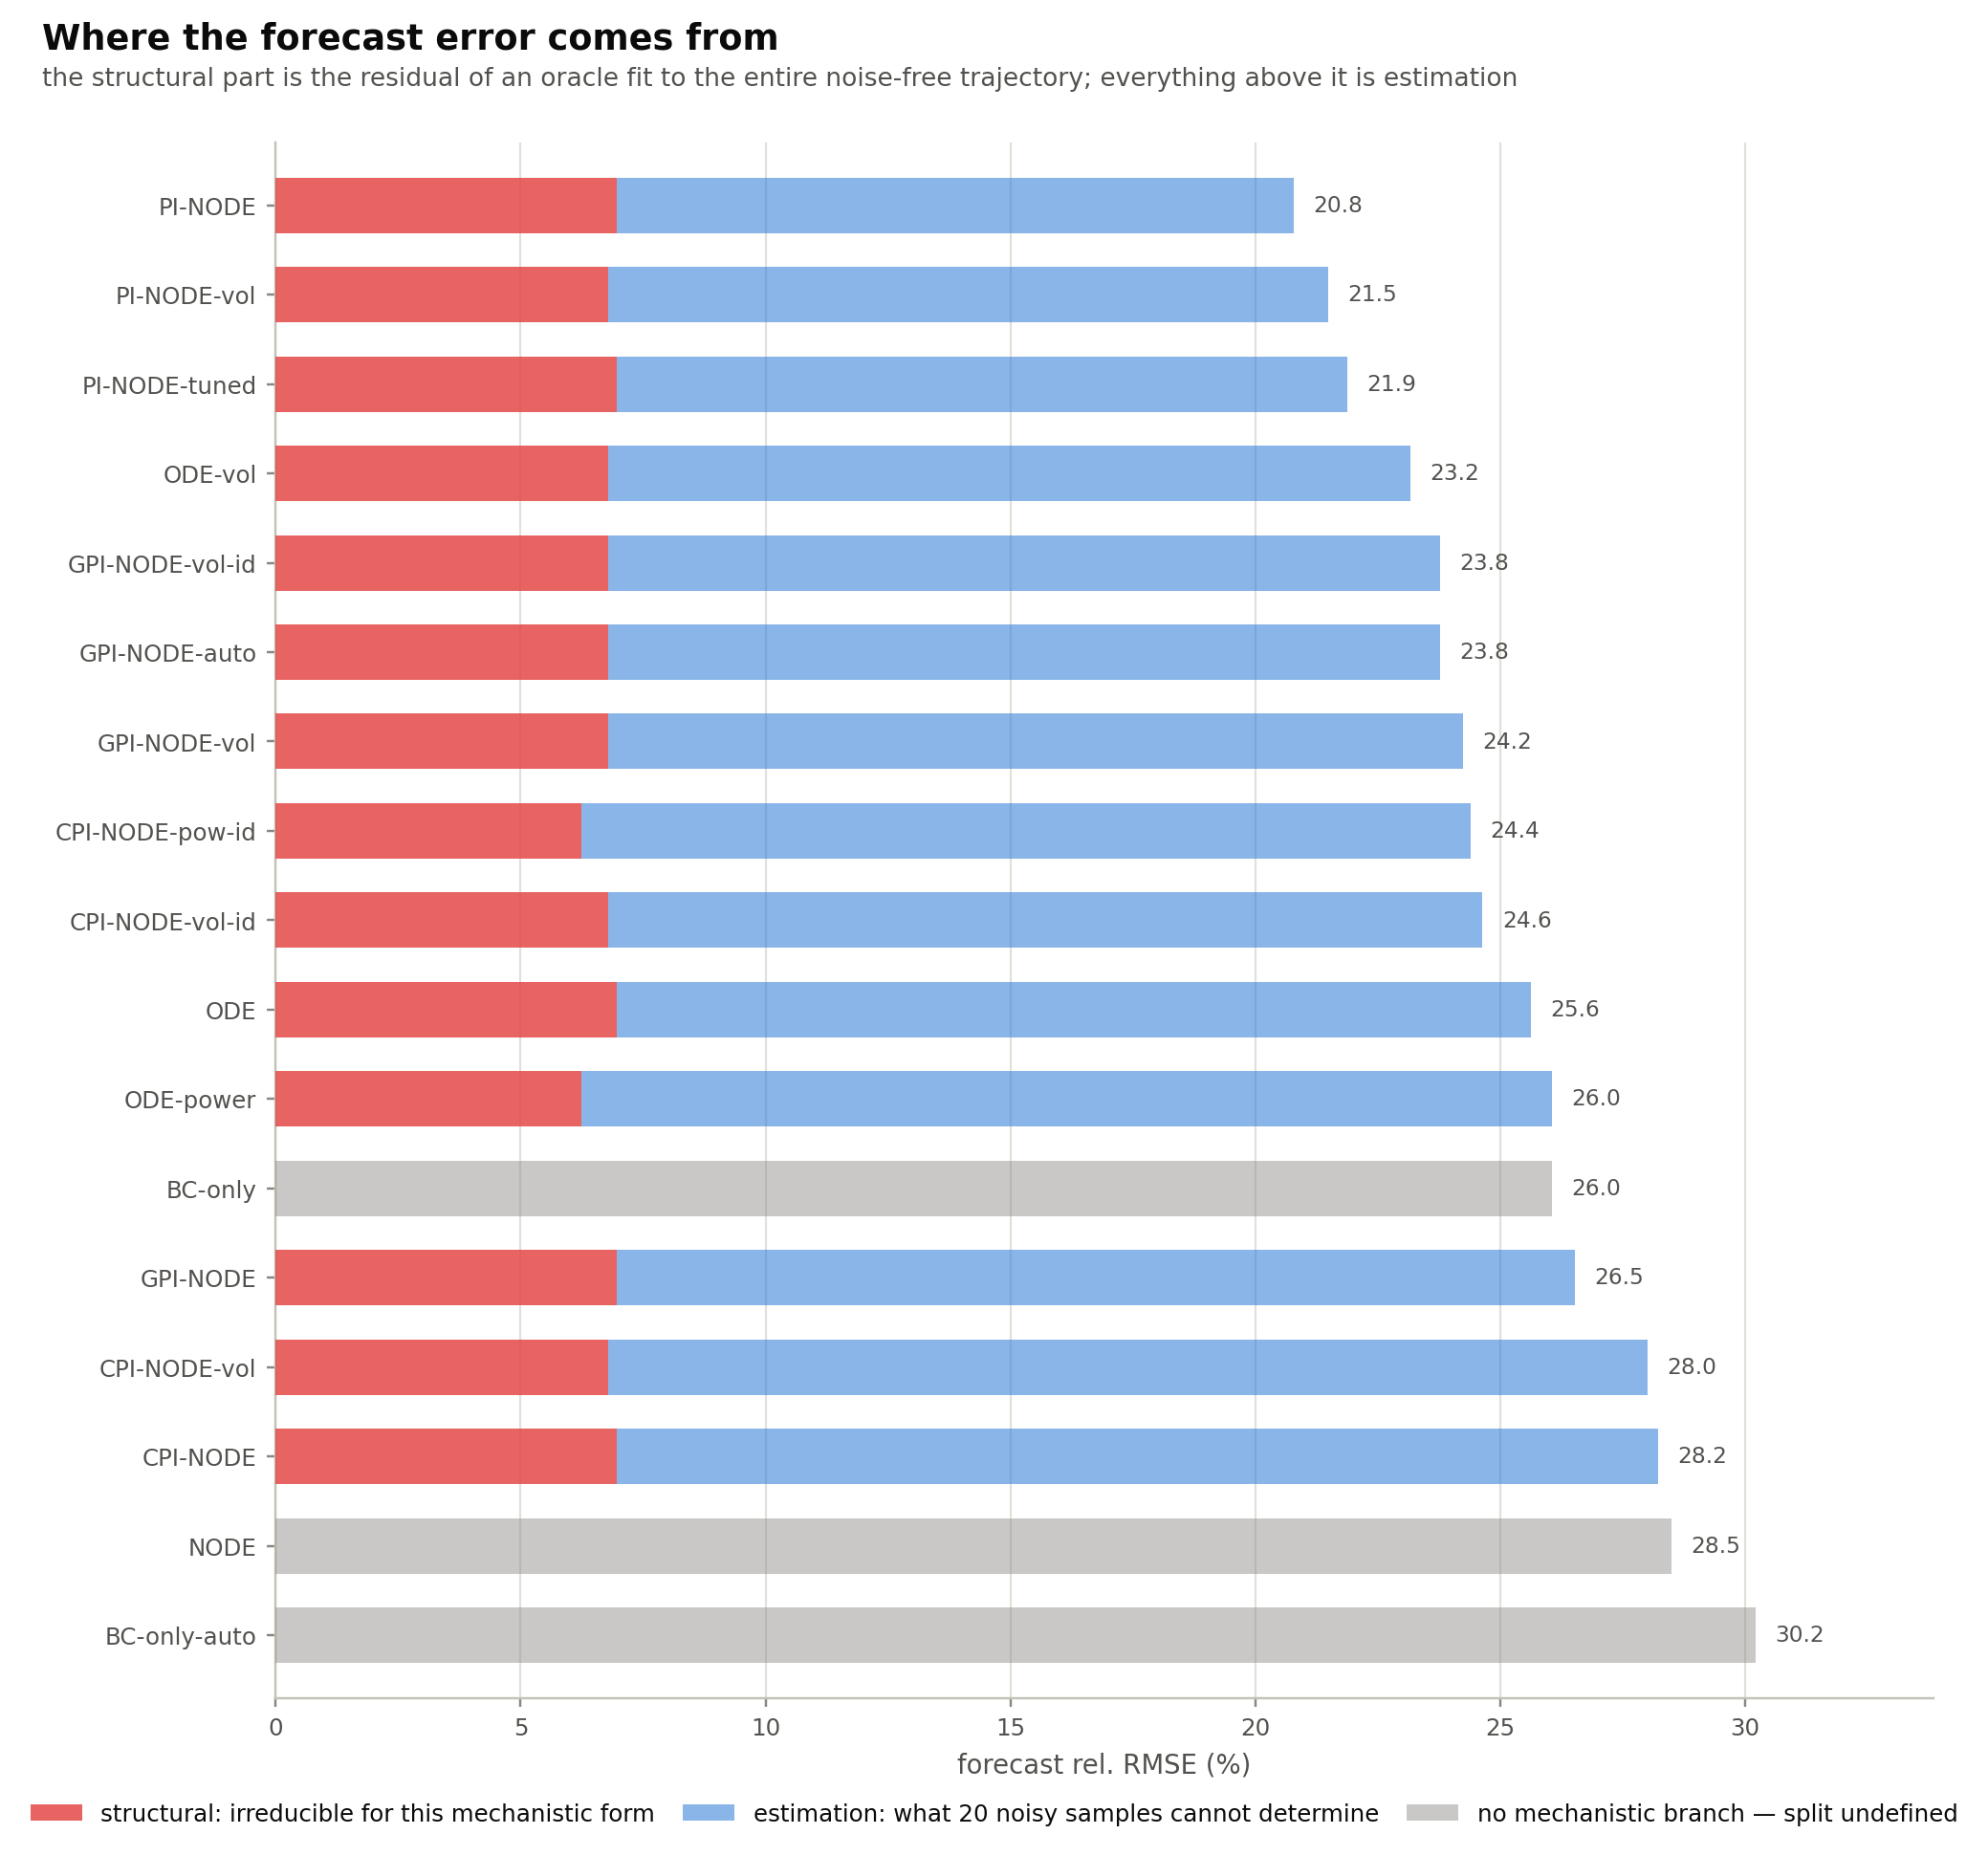
\includegraphics[width=0.95\textwidth]{figures/f9_error_budget.png}
\caption{Decomposition of the forecast error. The structural part is the
residual of an oracle fit to the entire noise-free trajectory --- the best the
model form can do with no estimation error at all; everything above it is what
sparse noisy assimilation fails to determine.}
\label{fig:error_budget}\end{figure}

\begin{figure}[t]\centering
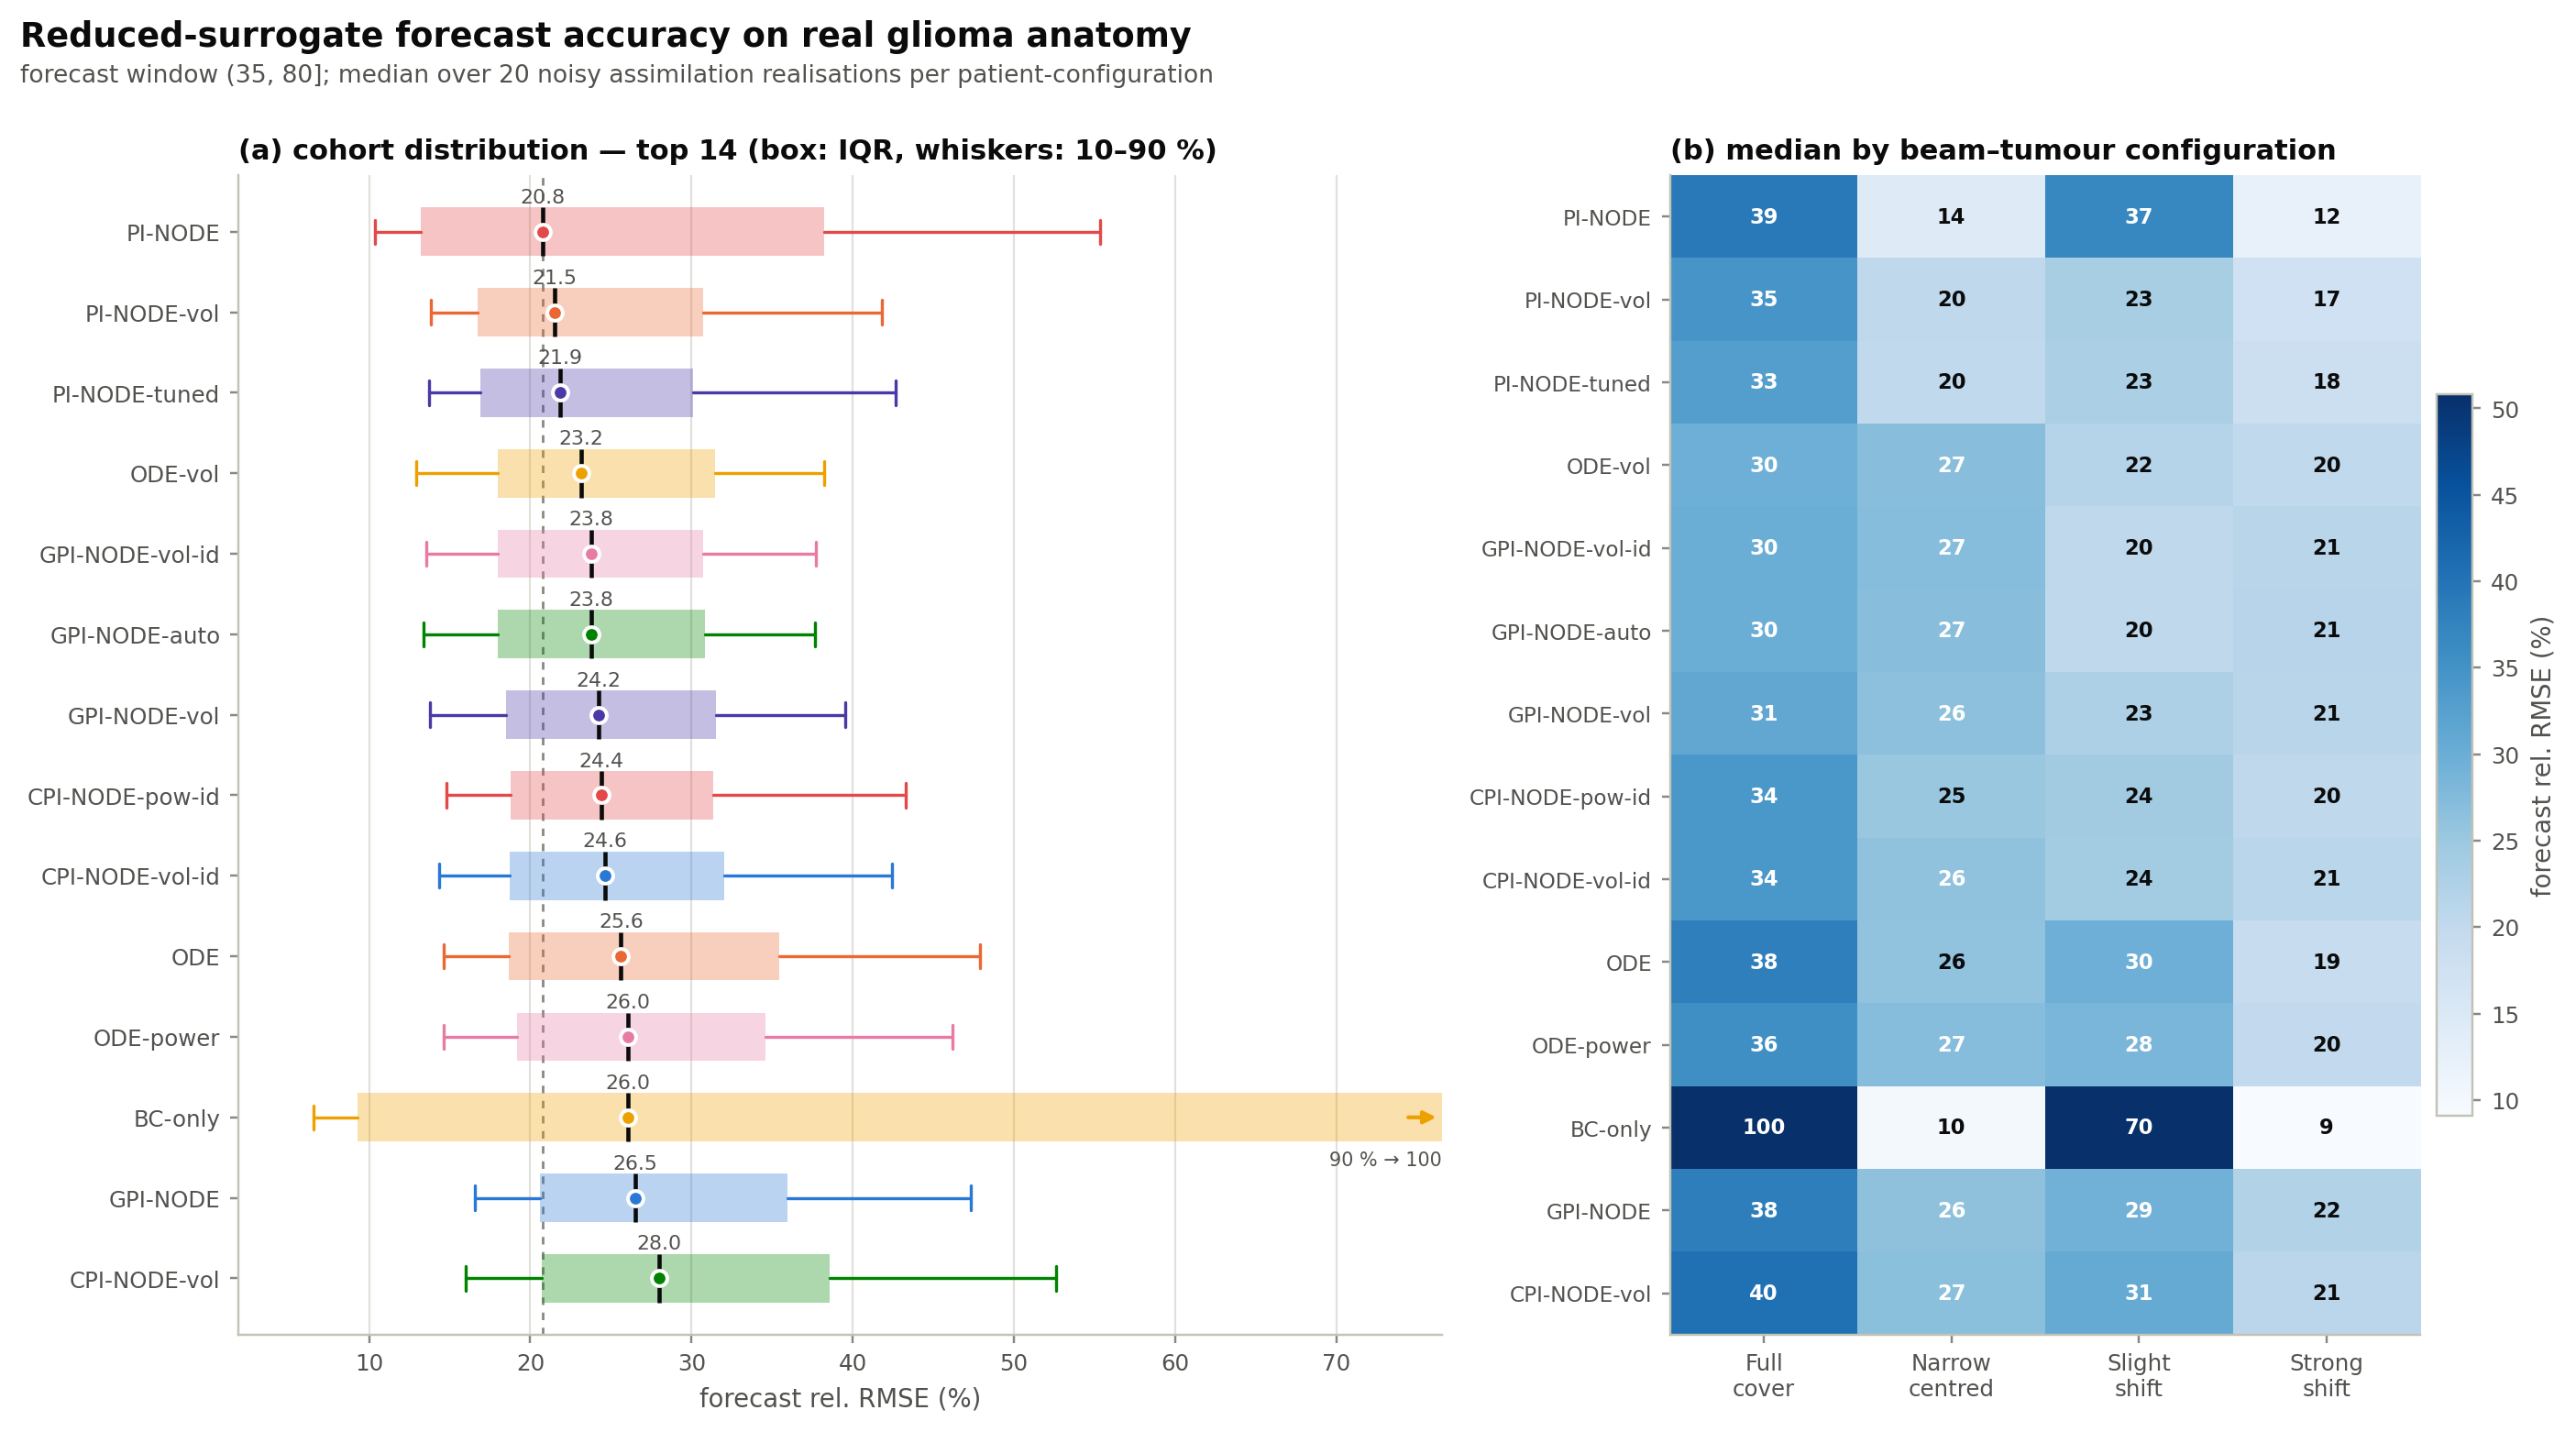
\includegraphics[width=1.0\textwidth]{figures/f8_cohort_accuracy.png}
\caption{Cohort distribution of the forecast error per surrogate, and its median
per irradiation geometry.}
\label{fig:cohort_accuracy}\end{figure}

\subsection{Is the Physics--Closure Weight a Real Control?}
\label{sec:results_weights}

Section~\ref{sec:gauge} shows $(\omega,s_r)$ cannot be normalised. This section
asks the operational question instead: does the nominal weight predict the
balance the fitted model actually adopts? We sweep both parameterisations on the
same backbone and compare the nominal machine-learning share ---
$s_r/(\omega+s_r)$ for Eq.~\eqref{eq:pinode_weighted}, $\lambda$ for
Eq.~\eqref{eq:cpinode} --- against the realised share $1-\bar\Phi$ of
Eq.~\eqref{eq:phi}.

\begin{table}[H]
\caption{Nominal versus realised machine-learning share. $|\Delta|$ is the
calibration error.}
\label{tab:weights}
\centering\scriptsize
\setlength{\tabcolsep}{4pt}
%
\begin{tabular}{llrrrr}
\hline
\textbf{Parameterisation} & \textbf{Setting} & \textbf{nominal} & \textbf{realised} & $\bm{|\Delta|}$ & \textbf{Test (\%)} \\
\hline
$\omega f_{RT}+s_r g_\psi$ & $\omega{=}$1, $s_r{=}$0.02 & 0.020 & 0.459 & 0.439 & 37.31 \\
 & $\omega{=}$0.5, $s_r{=}$0.02 & 0.038 & 0.413 & 0.374 & 25.20 \\
 & $\omega{=}$1, $s_r{=}$0.05 & 0.048 & 0.475 & 0.427 & 37.73 \\
 & $\omega{=}$0.2, $s_r{=}$0.02 & 0.091 & 0.609 & 0.518 & 20.13 \\
 & $\omega{=}$0.5, $s_r{=}$0.05 & 0.091 & 0.461 & 0.370 & 27.88 \\
 & $\omega{=}$1, $s_r{=}$0.1 & 0.091 & 0.483 & 0.392 & 37.02 \\
 & $\omega{=}$0.5, $s_r{=}$0.1 & 0.167 & 0.480 & 0.314 & 29.02 \\
 & $\omega{=}$1, $s_r{=}$0.2 & 0.167 & 0.489 & 0.322 & 37.07 \\
 & $\omega{=}$0.2, $s_r{=}$0.05 & 0.200 & 0.623 & 0.423 & 21.49 \\
 & $\omega{=}$0.05, $s_r{=}$0.02 & 0.286 & 0.821 & 0.535 & 15.09 \\
 & $\omega{=}$0.5, $s_r{=}$0.2 & 0.286 & 0.494 & 0.208 & 28.45 \\
 & $\omega{=}$0.2, $s_r{=}$0.1 & 0.333 & 0.628 & 0.294 & 23.50 \\
 & $\omega{=}$0.02, $s_r{=}$0.02 & 0.500 & 0.900 & 0.400 & 14.47 \\
 & $\omega{=}$0.05, $s_r{=}$0.05 & 0.500 & 0.816 & 0.316 & 18.96 \\
 & $\omega{=}$0.2, $s_r{=}$0.2 & 0.500 & 0.630 & 0.130 & 23.60 \\
 & $\omega{=}$0.05, $s_r{=}$0.1 & 0.667 & 0.814 & 0.148 & 21.38 \\
 & $\omega{=}$0.02, $s_r{=}$0.05 & 0.714 & 0.897 & 0.183 & 18.65 \\
 & $\omega{=}$0.05, $s_r{=}$0.2 & 0.800 & 0.814 & 0.014 & 23.10 \\
 & $\omega{=}$0.02, $s_r{=}$0.1 & 0.833 & 0.896 & 0.063 & 22.19 \\
 & $\omega{=}$0.02, $s_r{=}$0.2 & 0.909 & 0.899 & 0.010 & 25.45 \\
\hline
$(1{-}\lambda)f_{RT}+\lambda\sigma\tanh g_\psi$ & $\lambda{=}$0 & 0.000 & 0.000 & 0.000 & 23.17 \\
 & $\lambda{=}$0.1 & 0.100 & 0.355 & 0.255 & 28.67 \\
 & $\lambda{=}$0.2 & 0.200 & 0.418 & 0.218 & 29.80 \\
 & $\lambda{=}$0.2 & 0.200 & 0.398 & 0.198 & 29.25 \\
 & $\lambda{=}$0.3 & 0.300 & 0.424 & 0.124 & 29.41 \\
 & $\lambda{=}$0.4 & 0.400 & 0.412 & 0.012 & 28.00 \\
 & $\lambda{=}$0.4 & 0.400 & 0.384 & 0.016 & 26.29 \\
 & $\lambda{=}$0.5 & 0.500 & 0.413 & 0.087 & 25.71 \\
 & $\lambda{=}$0.6 & 0.600 & 0.445 & 0.155 & 24.06 \\
 & $\lambda{=}$0.6 & 0.600 & 0.427 & 0.173 & 23.36 \\
 & $\lambda{=}$0.7 & 0.700 & 0.519 & 0.181 & 22.95 \\
 & $\lambda{=}$0.8 & 0.800 & 0.615 & 0.185 & 21.58 \\
 & $\lambda{=}$0.8 & 0.800 & 0.600 & 0.200 & 23.39 \\
 & $\lambda{=}$0.9 & 0.900 & 0.726 & 0.174 & 20.19 \\
 & $\lambda{=}$1 & 1.000 & 1.000 & 0.000 & 26.05 \\
 & $\lambda{=}$1 & 1.000 & 1.000 & 0.000 & 30.21 \\
\hline
\end{tabular}

\end{table}

Both parameterisations are monotone --- a larger nominal share does produce a
larger realised share (Spearman +0.89 and +0.94 respectively)
--- so both are usable as a dial. They differ in whether the dial is
\emph{calibrated}: the mean calibration error is 0.294 for
$(\omega,s_r)$ against 0.124 for $\lambda$, a factor of
2.4. Under Eq.~\eqref{eq:pinode_weighted} a setting whose nominal
machine-learning contribution is a few per cent can realise nearly half the
vector field, and settings whose nominal shares differ several-fold can land on
the same realised balance. Under Eq.~\eqref{eq:cpinode} the number on the dial
is, to within a few per cent, the share the model adopts, and the two endpoints
are exact --- $\lambda=0$ reproduces the assimilated mechanistic model to the
last digit even with a fully trained closure present (verified at
$0$).

\paragraph{Two consequences that are not merely about labelling.}
First, the published default is not the best cell of its own grid: sweeping
$(\omega,s_{r})$ finds $\omega{=}$0.02, $s_r{=}$0.02 at 14.47\,\% against
20.78\,\% for $(0.05,0.10)$, a \emph{32\,\% relative} improvement from
tuning alone. Second, and more informative, the winning cell has a realised
machine-learning share of 0.90: accuracy improves monotonically as
the realised physics share falls, so on this benchmark the formulation works
best as a lightly-anchored neural ODE rather than as a balanced hybrid. It is
worth stating plainly what the published numbers mean --- $(\omega,s_r) =
(0.05,0.10)$ reads as ``5\,\% physics, 10\,\% residual'' and is in fact
$81\,\%$ machine learning.

\paragraph{The original parameterisation cannot reach a physics-dominated
model.} Across the whole $5\times4$ grid the realised machine-learning share
spans only 0.41--0.90 (range 0.49), never
approaching either endpoint; the convex control spans the full
0.00--1.00. This is an expressiveness limitation, not
just an interpretability one: no choice of $(\omega,s_{r})$ in this range yields
the mechanistic model, even though $s_{r}=0$ nominally should.

\begin{figure}[t]\centering
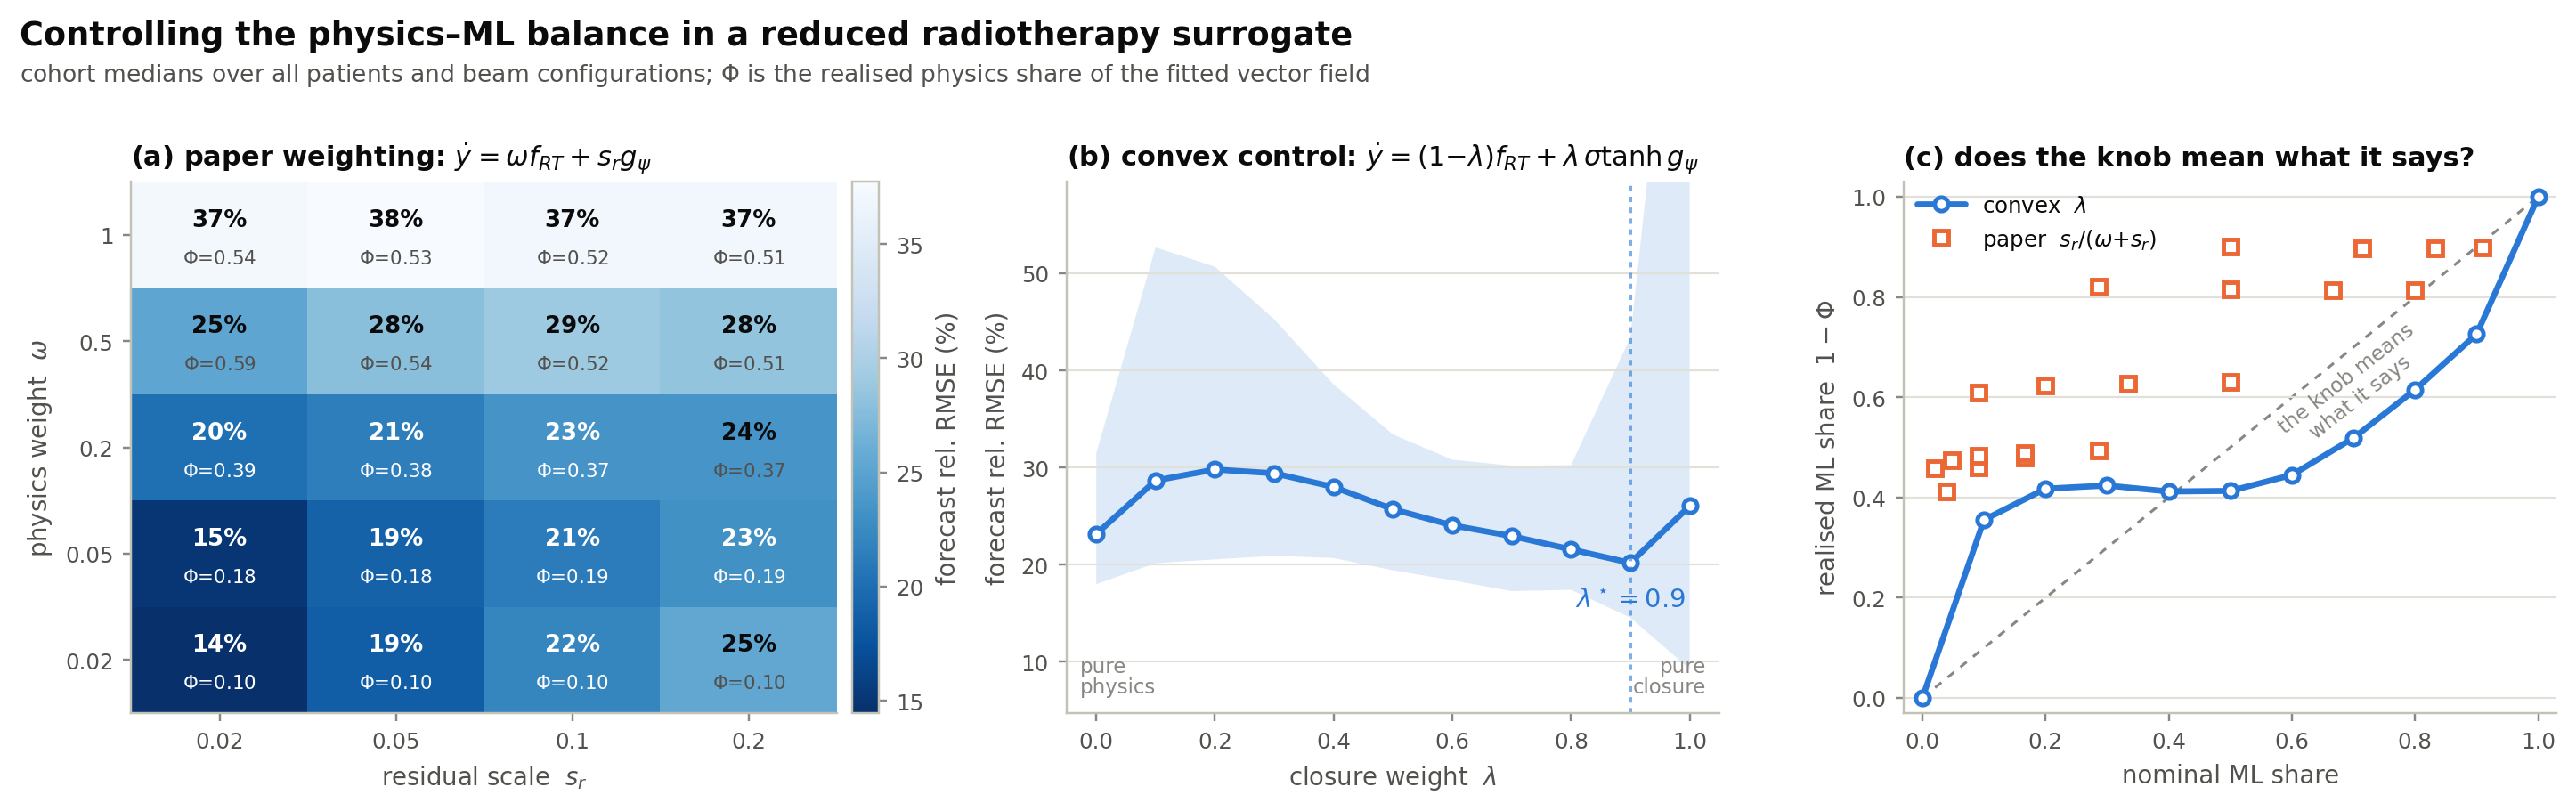
\includegraphics[width=1.0\textwidth]{figures/f6_weight_control.png}
\caption{(a) Forecast error over the $(\omega,s_r)$ grid of
Eq.~\eqref{eq:pinode_weighted}, with the realised physics share $\Phi$ printed
in each cell. (b) The same sweep for the single convex control $\lambda$ of
Eq.~\eqref{eq:cpinode}. (c) Realised against nominal machine-learning share for
both; the diagonal is perfect calibration.}
\label{fig:weight_control}\end{figure}

This is the practical answer to the question the two weights raise. They cannot
be made to sum to one, because both branches are cones and any normalisation is
undone by the branch's own parameters. Replacing them by a bounded closure, an
anchored backbone and an orthogonality constraint restores a single coefficient
that behaves like an interpolation weight, admits classical linear interpolation
between the mechanistic and learned models, and --- unlike $(\omega,s_r)$ ---
can be reported and compared across studies. Given
Section~\ref{sec:results_main}, the coefficient that matters is not a global
constant but the gate of Eq.~\eqref{eq:gate}; the value of making it
identifiable is that its output is then a meaningful readout of \emph{where}
the reduced physics is failing.

\subsection{Can a Learned Gate Recover the Regime-Dependent Optimum?}
\label{sec:results_gate}

Section~\ref{sec:results_main} shows the optimal balance inverts with the
irradiation geometry, and Eq.~\eqref{eq:gate} is the natural response: let
$\lambda$ depend on the state and discover the schedule. Table~\ref{tab:gate}
tests it by varying how strongly the gate is restrained.

\begin{table}[H]
\caption{Gate ablation. $\eta$ is the penalty on the trajectory-averaged gate;
the identifiability rows use $\eta = 0.02$ and add the anchor and orthogonality
terms of Section~\ref{sec:convex} singly and together.}
\label{tab:gate}
\centering\scriptsize
\setlength{\tabcolsep}{5pt}
\begin{tabular}{lrrr}
\hline
\textbf{Variant} & \textbf{Test (\%)} & \textbf{IQR} & $\bm{\bar\Phi}$ \\
\hline
orthogonality only & \textbf{23.5} & 12.2 & 0.97 \\
gate penalty $\eta = 0.3$ & 23.7 & 12.8 & 0.99 \\
anchor + orthogonality + warm start & 23.8 & 12.8 & 1.00 \\
anchor only & 23.9 & 12.9 & 0.97 \\
$\eta = 0.08$ & 24.0 & 13.0 & 0.98 \\
no identifiability terms ($\eta = 0.02$) & 24.2 & 13.0 & 0.93 \\
$\eta = 0.005$ & 27.4 & 14.5 & 0.78 \\
$\eta = 0$ (free gate) & 29.0 & 28.8 & 0.67 \\
\hline
\end{tabular}
\end{table}

The relationship is monotone, and it runs against the hypothesis: \emph{the more
authority the gate takes, the worse the forecast.} A completely free gate settles
at $\bar\Phi\approx0.67$ \emph{uniformly} --- the damaging interior regime ---
and posts the worst result in the group, with three times the spread of the
restrained variants and $52\,\%$ error on the covered configurations.

\paragraph{The natural diagnosis is observability, and it is wrong.}
The reduced state $(y,z,t,U)$ cannot distinguish an under-sized field from a
displaced one, so an obvious explanation is that the gate has no way to know
which regime it is in. We tested this directly by giving the gate the one scalar
that does separate them --- the mass-weighted dose coverage at $t=0$, which any
treatment plan reports without additional measurement. The closure never
receives it, so identifiability is unaffected. The result is a null
(Table~\ref{tab:context}): with and without the signal the forecast error agrees
to within $0.24$ percentage points and the realised shares are identical to two
decimals. The gate ignores the information.

\begin{table}[H]
\caption{Handing the gate an explicit regime signal (dose coverage at $t=0$)
changes nothing. Forecast relative RMSE (\%), full cohort.}
\label{tab:context}
\centering\scriptsize
\setlength{\tabcolsep}{6pt}
\begin{tabular}{rrrr}
\hline
$\bm{\eta}$ & \textbf{gate with coverage} & \textbf{gate without} & $\bm{\Delta}$ \\
\hline
0 & 28.42 & 28.45 & $-0.03$ \\
0.005 & 27.02 & 27.02 & $0.00$ \\
0.02 & 23.73 & 23.80 & $-0.07$ \\
0.08 & \textbf{23.12} & 23.36 & $-0.24$ \\
\hline
\end{tabular}
\end{table}

\paragraph{The schedule has no in-window signature.}
The explanation is in the training column of Table~\ref{tab:gate}: it is flat at
$1.3$--$1.6\,\%$ --- the observation-noise floor --- while the forecast error
moves from $29.0\,\%$ to $23.7\,\%$. Every setting of the gate fits the
assimilation window equally well. The regime distinction pays only in the
forecast window, which the objective never sees, so no gate can learn a
forecast-improving schedule from an in-window loss, however it is parameterised
and whatever side information it is given. The gate does not lack information;
it lacks a reason to use it. The penalty $\eta$ helps monotonically precisely
because it substitutes an explicit prior for a signal the loss cannot supply.

This sharpens the ambiguity measured in Fig.~\ref{fig:ground_truth}(c). That
window-indistinguishable trajectories diverge afterwards is not only why a
closure term is needed --- it is why the closure's schedule cannot be fitted.

The same tables correct a natural mis-attribution. Within the gated family the
identifiability terms \emph{improve} accuracy --- $24.2\,\%$ without them,
$23.5\,\%$ with the orthogonality projection alone. The accuracy cost identified
in Section~\ref{sec:results_weights} is not the anchor or the projection; it is
the $\tanh$ \emph{bound}, which is precisely the ingredient that removes the
$s_{r}$ gauge.

\paragraph{Consequence: set the balance, do not learn it.} The physics--closure
balance is a plan-time decision. The treatment geometry is known before any
response data exists, the right choice is worth a factor of two to three
(Section~\ref{sec:results_main}), and a conformal well-covering field calls for
a physics-dominated surrogate while an under-sized or displaced one calls for
closure authority. Learning the schedule instead would require an objective that
can see the payoff --- a forecast-window loss, and therefore a longitudinal
cohort with a post-treatment observation. That is a data-collection requirement,
not a modelling one.

\begin{figure}[t]\centering
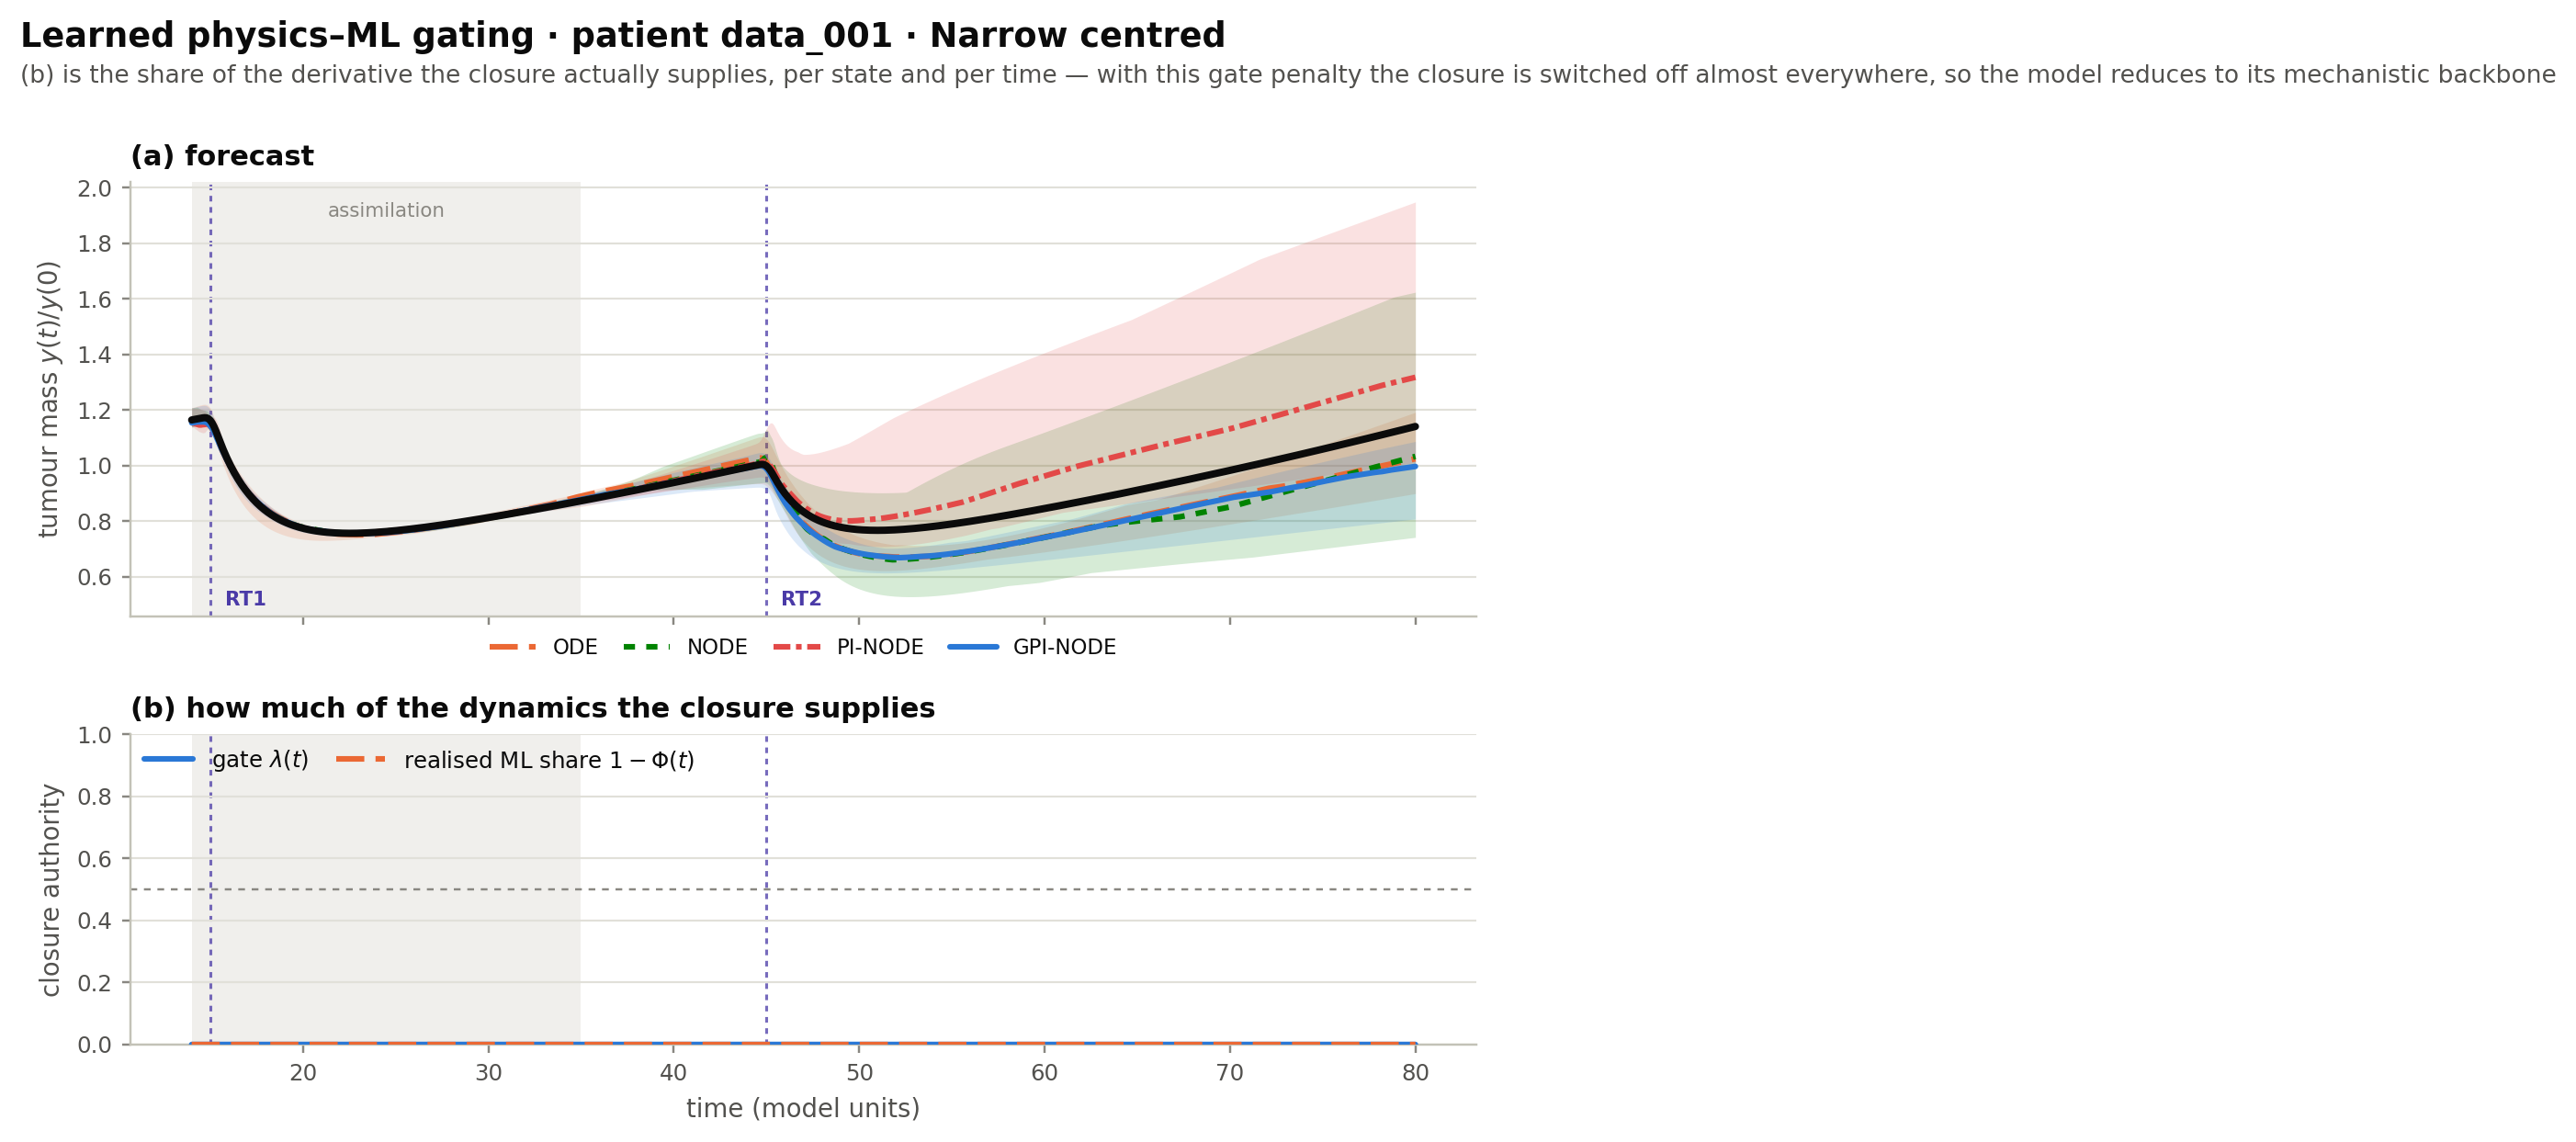
\includegraphics[width=0.85\textwidth]{figures/f7_gate.png}
\caption{The learned gate of Eq.~\eqref{eq:gate}: the forecast, and the share of
the derivative the closure actually supplies as a function of time. At the gate
penalty used here the closure is switched off almost everywhere and the model
reduces to its mechanistic backbone --- a faithful readout of what the fit
chose, and the reason the identified variant forfeits the closure advantage
available on the mismatched geometries.}
\label{fig:gate}\end{figure}

\subsection*{Summary of Changes to the Model Equations}
\label{sec:changes}

For clarity, Table~\ref{tab:changes} records every modification made to the
reduced formulation, why it was needed, and what it establishes. Each is derived
in the section indicated.

\begin{table}[H]
\caption{Modifications to the reduced surrogate equations.}
\label{tab:changes}
\centering\scriptsize
\setlength{\tabcolsep}{3pt}
\renewcommand{\arraystretch}{1.15}
\begin{tabular}{p{2.3cm} p{3.4cm} p{2.9cm} p{3.1cm}}
\hline
\textbf{Original} & \textbf{Modified} & \textbf{Why} & \textbf{What it achieves} \\
\hline

$\dot y=\rho y(1-y/K)-\gamma zy-\mu y$
\newline Eq.~\eqref{eq:ode_rt_2state}
&
$\dot y=\rho y^{q}(1-y/K)-\gamma zy-\mu y$
\newline Eq.~\eqref{eq:backbone_q}
&
A constant-speed invasion front gives $y\sim(a+bt)^{3}$, hence
$\dot y\propto y^{2/3}$, not $y$ (Section~\ref{sec:volumetric})
&
The cheapest improvement available: no extra parameters, no network,
no extra training. 25.62\,\%\,$\to$\,23.17\,\%, and it cuts the
PI-NODE's spread across the cohort by 44\,\%. Empirical exponent $0.81$
\\
\hline

$\dot y=\omega f_{RT}+s_{r}g_{\psi}$
\newline Eq.~\eqref{eq:pinode_weighted}
&
$\dot y=(1-\lambda)f_{RT}+\lambda\sigma_{\mathrm{ref}}\tanh g_{\psi}$
\newline Eq.~\eqref{eq:cpinode}
&
$\omega$ and $s_{r}$ are exact gauge freedoms; both branches are cones, so no
normalisation exists (Section~\ref{sec:gauge})
&
A single identifiable, calibrated coefficient: calibration error
0.294\,$\to$\,0.124. Exact endpoints; linear interpolation becomes
meaningful
\\
\hline

--- (new)
&
$w_{\theta}\|\log(\theta/\theta_{\mathrm{ref}})\|^{2}$
&
Without it $(1-\lambda)$ is reabsorbed into $\theta$ and $\lambda$ is a gauge
again (verified at $1.6\times10^{-16}$)
&
Fixes the physics amplitude so $\lambda=0$ is \emph{the} assimilated
mechanistic model, not a rescaled copy
\\
\hline

--- (new)
&
$w_{\perp}\|P_{\mathrm{span}(\partial f/\partial\theta)}\tanh g_{\psi}\|^{2}$
&
A closure lying in the span of the parameter sensitivities is silently
re-estimating $\theta$
&
Identifies the physics--closure \emph{ratio}, and directly prevents the
distorted-effective-parameter failure this work targets
\\
\hline

$\lambda$ constant
&
$\lambda(y,z,t,U)=\sigma(h_{\xi}+\beta_{0})$
\newline Eq.~\eqref{eq:gate}
&
The reduced physics is adequate in some regimes and not others
(Section~\ref{sec:gate})
&
Lets the closure act only where the physics fails; the penalty $\eta$ sets how
readily it does so
\\
\hline

--- (new diagnostic)
&
$\Phi=|\dot y_{\mathrm{phys}}|/(|\dot y_{\mathrm{phys}}|+|\dot y_{\mathrm{ML}}|)$
\newline Eq.~\eqref{eq:phi}
&
A nominal weight need not equal the balance a fitted model adopts
&
Puts both parameterisations on one axis and makes the calibration claim testable
rather than assumed
\\
\hline
\end{tabular}
\end{table}

Two further changes concern the experimental procedure rather than the model,
but affect every number reported:
the integration grid used during assimilation is fixed and refined around the
dose pulses, rather than being the sparse observation grid itself, so a fitted
parameter cannot depend on how densely the tumour happened to be measured; and
the assimilation window begins at $t=14$ rather than $t=15$, so that it brackets
the first fraction instead of beginning on it and the surrogate is not required
to infer a latent damage state it was never shown.
